%!TEX TS-program = ../make.zsh

\begin{frame}[fragile]{Project status}

  \begin{columns}
    \begin{column}{0.5\textwidth}
      \begin{overlayarea}{\textwidth}{\textheight}
        \small
        \begin{itemize}
          \setlength\itemsep{0.2em}
          \item<alert@1>[\done] Implement new ray-tracing algorithm
          \item<alert@2>[\done] Implement hole ice and cables
          \item<alert@3>[\done] Verify plausibility with examples
          \item<alert@4>[\done] Verify with statistical cross checks
          %\item<alert@5>[\done] Compare to effective descriptions
          \item<alert@5>[\done] Bring interface up to date with current icetray %(September 2022)
          \item<alert@6>[\done] Provide python-3 example scripts \& documentation
          \item<alert@7>[\done] Provide steamshovel artists
          \item<alert@8>[\inprogress] Fix compatibility issues with
          \begin{itemize}
            \item[\tobedone] ice tilt, ice anisotropy
            \item[\tobedone] bfr
            \item[\tobedone] direct detection
          \end{itemize}
          \item<alert@9>[\tobedone] Convenient subclassing
          \item<alert@10>[\tobedone] Implement detection-probability property
        \end{itemize}
      \end{overlayarea}
    \end{column}
    \begin{column}{0.5\textwidth}%
      \only<1>{\image{how-does-it-work-004}}%
      \only<2>{\image{cable-inside-shifted-bc-steamshovel}}%
      \only<3>{
        \begin{center}
          %\hspace{10mm}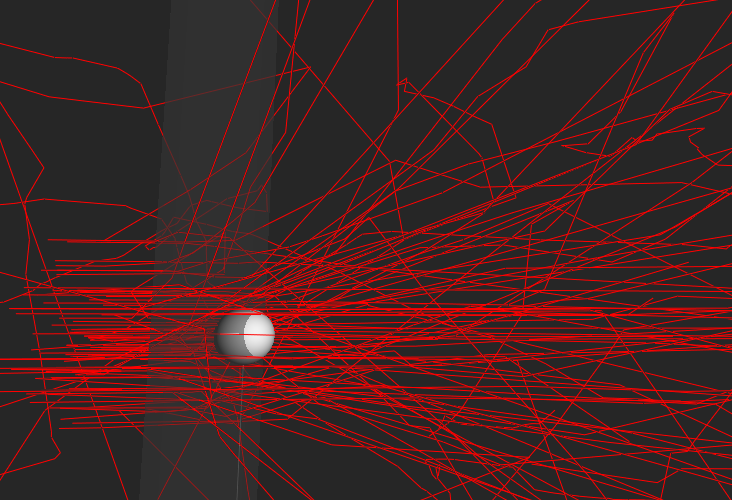
\includegraphics[width=0.8\textwidth]{img/asymmetry-example-steamshovel}
          %\image{asymmetry-example-angular-acceptance-with-comment}
          \vspace*{-1cm}
          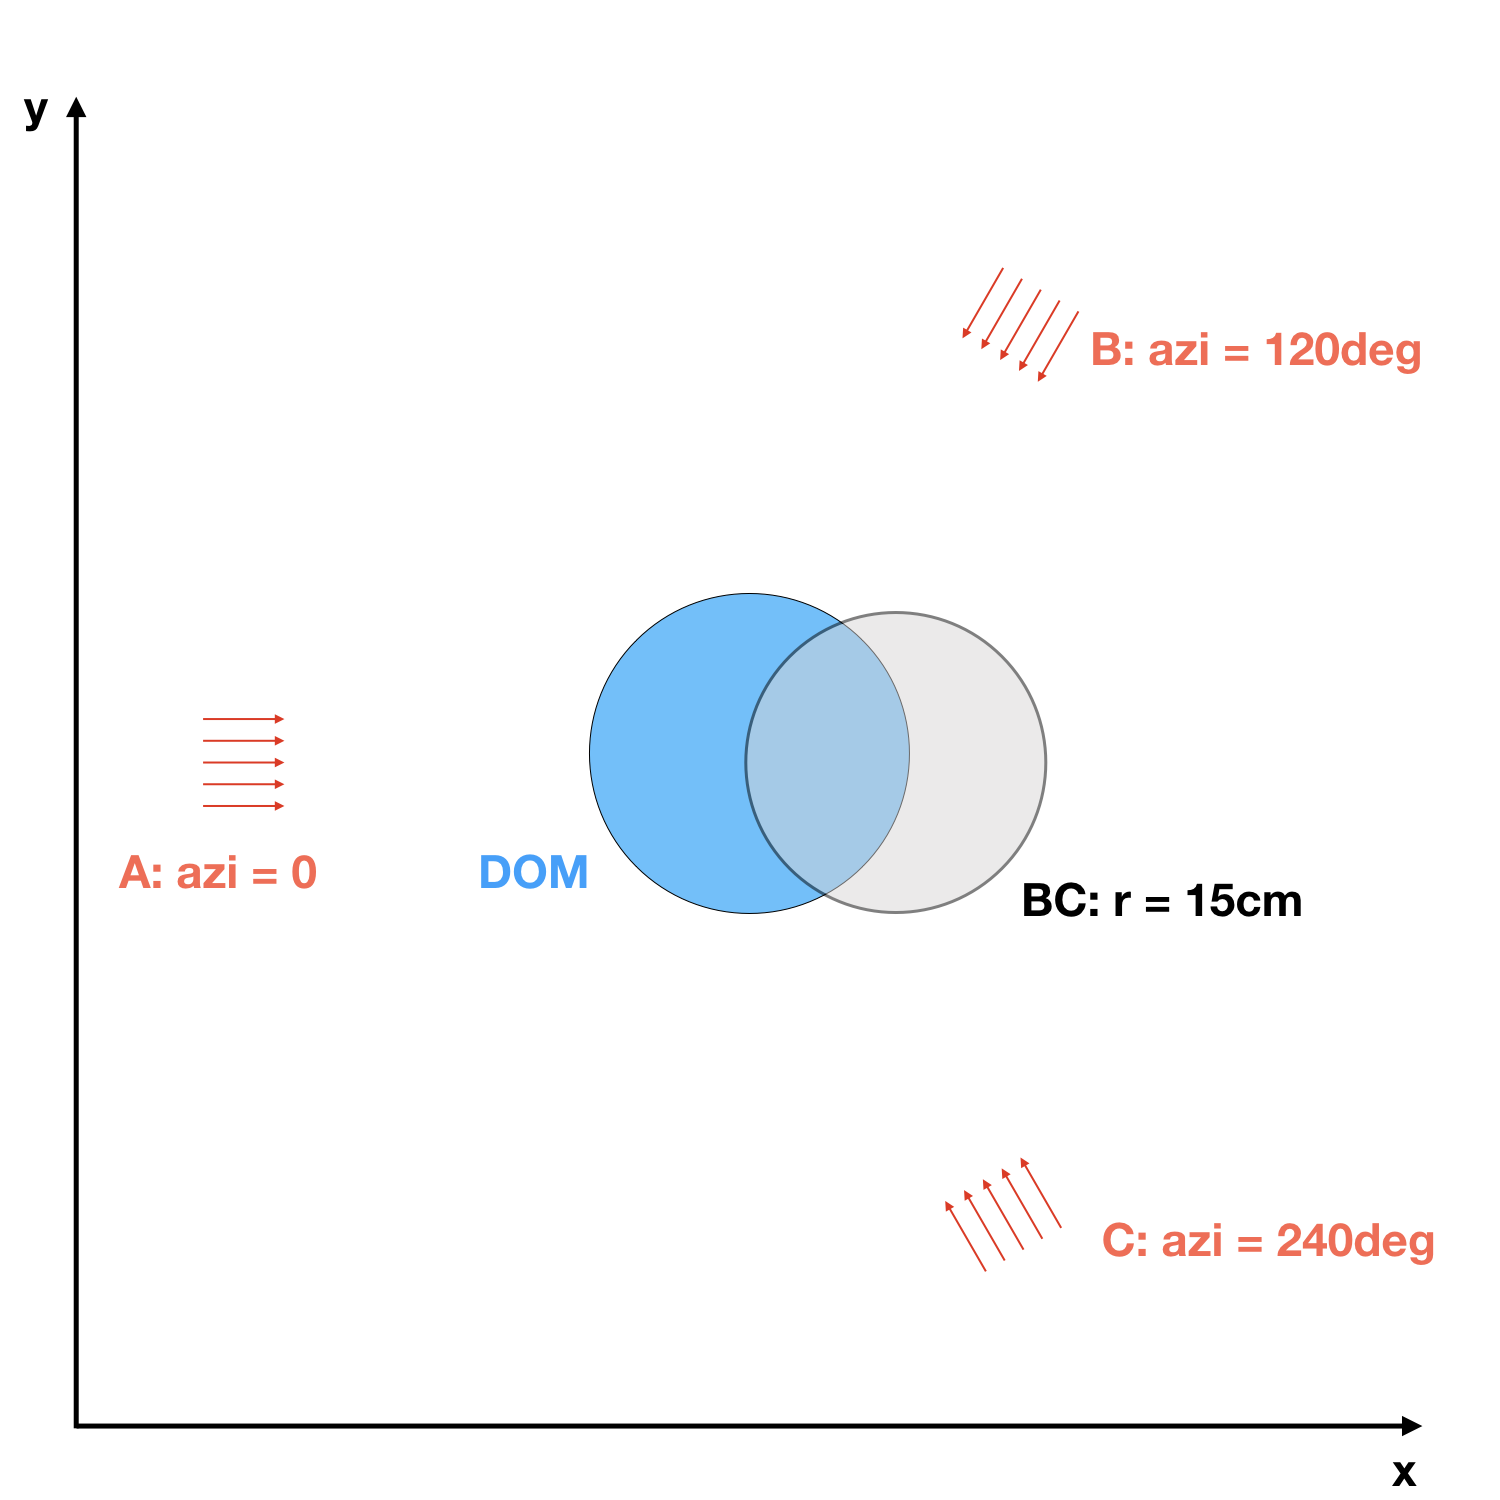
\includegraphics[width=0.6\textwidth]{img/summerscenario-004}
          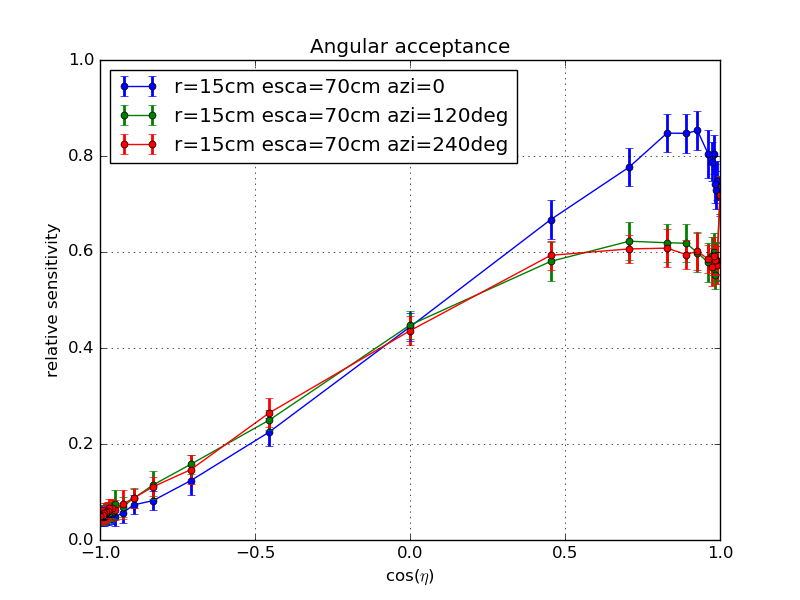
\includegraphics[width=0.8\textwidth]{img/summer_scenario_r15cm_esca70cm}
        \end{center}
      }%
      \only<4>{
        \image{cross-check-66-path-length-histogram}

        \tiny See also: \url{https://github.com/fiedl/hole-ice-study/issues/66}
      }%
      %\only<5>{
      %  \image{ppc-pocam-3}
      %
      %  \tiny See also: \url{https://github.com/fiedl/hole-ice-study/issues/4}, \url{https://github.com/fiedl/hole-ice-study/labels/comparison}
      %
      %  \normalsize
      %  \vspace{2em}
      %
      %  \metroset{block=fill}
      %  \begin{block}{Thesis \& previous talks}
      %    %$\rightarrow$ Thesis \& previous talks: \\
      %    \url{https://arxiv.org/abs/1904.08422} \\
      %    \scriptsize \url{https://github.com/fiedl/hole-ice-talk/releases}
      %  \end{block}
      %}%
      \only<5>{
        Ported to icetray main branch of September 2022.
        
        \vspace{1.5cm}
        
        \metroset{block=fill}
        \begin{block}{Pull request draft}
          \url{https://github.com/icecube/icetray/pull/2957}
        \end{block}
      
      }%
      \only<6>{
        Example scripts for new interface:
        \vspace{1cm}
        
        \metroset{block=fill}
        \begin{block}{Repository}
          \url{https://github.com/fiedl/hole-ice-scripts}
        \end{block}
      }%
      \only<7>{%
        Ready-to-use steamshovel artists included in pull request.
        \vspace{1cm}

        \image{config-example-steamshovel-3}
      }
      \only<9>{%
        \small\hspace*{-2cm}\vspace*{-1cm}
        \begin{forest}
          [I3CLSimMediumShape
            [I3CLSimMediumSphere]
            [I3CLSimMediumCylinder
              [I3CLSimHoleIceCylinder]
              [I3CLSimCableCylinder]
            ]
          ]
        \end{forest}
      }%
      \only<10>{%
        \image{dom_types_with_shapes}
      }%
    \end{column}
  \end{columns}

\end{frame}